\chapter{Implementation}\label{chapter:implementation}

This chapter describes the Python prototype that implements the reference
architecture from Chapter~\ref{chapter:design}. The prototype follows the
Pipes and Filters pattern: data moves through small processing stages, and
each stage performs one task before passing the result on~\cite{buschmann1996posa}.
This structure matches the pipeline roles introduced in
Figure~\ref{fig:pipeline-components}: collectors create data records,
transformers process records, dispatchers route them, converters prepare data
for checking, and verdict services produce verdicts.

The chapter first gives the technology choices and the code organization. It
then follows the runtime path of a record from collection to transformation,
export, checking, and verdict output. The final sections describe YAML
configuration, the verifier-side runtime, and generated deployment
configurations.

\section{Technology Choices and Code Organization}
\label{sec:impl-organization}

The prototype is implemented in Python. ROS~2 provides the Python client
library \texttt{rclpy}, which allows the monitor to join the ROS graph as a
normal node. Python also has runtime type utilities through
\texttt{rosidl\_runtime\_py}. These utilities resolve ROS~2 message, service,
and action classes from their type names, so a configured source can be
collected through runtime type resolution. Python also keeps
project-specific converters and verdict services simple to add.

Only the collector layer imports ROS~2 packages. The remaining modules use the
Python standard library, \texttt{PyYAML} for configuration parsing, and
\texttt{paho-mqtt} for MQTT transport. As a result, the verifier side of a
split deployment can run on a plain Python installation. If \texttt{paho-mqtt}
is unavailable, MQTT components are skipped at construction time while the rest
of the modules remain importable and testable.

The repository separates infrastructure code from project-specific checking
logic. The \texttt{monitor/} package contains the reusable monitoring
infrastructure. The \texttt{custom/} package contains converters and verdict
services used by the case studies. Table~\ref{tab:impl-modules} maps the main
modules in \texttt{monitor/} to the pipeline roles from
Chapter~\ref{chapter:design}.

\begin{table}[htbp]
\centering
\begin{tabular}{
    >{\raggedright\arraybackslash}p{0.34\textwidth}
    >{\raggedright\arraybackslash}p{0.56\textwidth}
}
\toprule
\textbf{Module} & \textbf{Responsibility} \\
\midrule
\texttt{monitor\_node.py} &
ROS~2-facing entry point for integrated and robot-side monitoring. \\
\texttt{node\_runner.py} &
ROS-free entry point for verifier-side processes. \\
\texttt{collector.py} &
Topic, service, and action collectors. \\
\texttt{data\_record.py} &
The common data record and its JSON serialization. \\
\texttt{transformer.py} &
Transformer pipeline and built-in transformers. \\
\texttt{exporter.py}, \texttt{exporters.py},
\texttt{exporter\_mqtt.py} &
Exporter interface, dispatcher, file exporter, and MQTT exporter. \\
\texttt{source.py}, \texttt{sources.py}, \texttt{source\_file.py},
\texttt{source\_mqtt.py} &
Verifier-side source interface, file replay source, and MQTT source. \\
\texttt{converter.py}, \texttt{verdict.py},
\texttt{verdict\_exporters.py} &
Converter and verdict-service base classes, verdict records, and verdict
exporters. \\
\texttt{dsl\_transport.py} &
File and MQTT transports for converter output. \\
\texttt{config\_model.py}, \texttt{pipeline.py},
\texttt{runtime\_builder.py} &
Typed configuration model and builders for runtime wiring. \\
\texttt{config\_gen.py} &
Generator that turns one deployment description into runtime configuration
files. \\
\bottomrule
\end{tabular}
\caption{Main modules of the \texttt{monitor/} package and their pipeline
responsibilities.}
\label{tab:impl-modules}
\end{table}

\section{The Monitor Process}
\label{sec:impl-monitor-process}

The monitor process is the ROS~2-facing runtime. It is used in the integrated
deployment and on the robot side of the split deployment. It is implemented in
\texttt{monitor\_node.py} as one ROS~2 node.

At startup, the process loads a YAML file into the typed configuration model.
It creates a session identifier from the current time and a short random
component, then builds the configured data exporters and the checking graph.
The process waits briefly for DDS discovery and reads the visible topic and
service names from the ROS graph. This discovered type information is used only
as a fallback. If a source type is already given in the configuration, that
configured type is used.

For each configured topic, service, or action, the process creates one
collector and one transformer pipeline. A source can also define its own
exporters. In that case, records from that source go to a source-specific
dispatcher. This is useful when, for example, one high-rate topic should be
sent to MQTT while other records are written to a file. All records are also
passed to the checking graph when one is configured.

Each run is marked with two session records. The first record is
\texttt{session\_start}; it contains the complete parsed configuration, so an
output file is self-contained for later interpretation. On
shutdown, collectors are stopped, a \texttt{session\_end} record with summary
statistics is emitted, and exporters are flushed and closed.

\section{Collecting ROS 2 Observations}
\label{sec:impl-collectors}

Collectors implement the observation mechanisms described in
Section~\ref{sec:observing-ros2}. They share a base class that owns the
per-source sequence counter, the transformer pipeline, and the export callback.
The concrete collectors differ in the ROS~2 entity they subscribe to.

\paragraph{Topics.} The topic collector resolves the configured message type
to a Python class at runtime. It then creates a normal ROS~2 subscription with
a configurable QoS depth. Each received message is converted to a dictionary
with \texttt{message\_to\_ordereddict}. The same collector code can therefore
handle any topic type that is available in the runtime environment.

\paragraph{Services.} The service collector subscribes to the event topic of
the configured service. Its name is formed by appending
\texttt{/\_service\_event} to the service name. This topic exists when service
introspection is enabled on the service client or server, as explained in
Section~\ref{sec:observing-services}. The collector derives the event message
class from the configured service type and subscribes with a reliable,
transient-local QoS profile. Each event is converted into a request or response
record. The event type determines the phase, the request or response payload
becomes the record data, and the client identifier and sequence number are kept
in the metadata for request-response correlation.

\paragraph{Actions.} The action collector subscribes to the hidden feedback
and status topics of the configured action:
\texttt{<action>/\_action/feedback} and
\texttt{<action>/\_action/status}. The feedback type is resolved from the
action type. The status topic uses the standard goal-status array message from
\texttt{action\_msgs}. The configured phases decide
whether feedback, status, or both are collected. Goal, result, and cancellation
exchanges use services inside ROS~2 actions. Service introspection handles those
phases, while the action collector handles feedback and status.

Collectors also try to record the source node that produced an observation.
DDS discovery may still be incomplete when the first message arrives. In that
case, ROS~2 can report a placeholder publisher name. The collectors retry
placeholder lookups on later callbacks and store the
node name once a real name is available. Until then, the record simply omits
the source-node field.

\section{Records and Transformers}
\label{sec:impl-records}

The common data record described in Table~\ref{tab:data-record-schema} is
implemented as a Python dataclass. It is the data unit that moves through the
pipeline. Each record stores the record kind, session identifier, source type,
source name, message type, timestamp, payload, and optional metadata.

Records are serialized as JSON Lines (JSONL), with one JSON object per line.
Empty optional fields are omitted. Deserialization restores the same record
fields, so records preserve their monitoring context across files and network
transports. A data record identifier combines the session
identifier, source type, source name, phase, and per-collector sequence number.
The identifier is unique within one session and remains readable in logs and
output files. The following shortened JSONL line shows a topic record after
field extraction:

\begin{small}
\begin{verbatim}
{"_type": "data", "session_id": "20260709_142401_5f2c31ab",
 "record_id": "20260709_142401_5f2c31ab:topic:/odom:-:17",
 "source_type": "topic", "source_name": "/odom",
 "msg_type": "nav_msgs/msg/Odometry", "timestamp": 1783002941.312,
 "data": {"twist.twist.linear.x": 0.62},
 "metadata": {"seq": 17, "transformers_applied":
              ["FieldExtractor", "RateThrottler"]}}
\end{verbatim}
\end{small}

Each collector sends its records through a transformer pipeline before they
are exported or checked. Transformers run in the order given in the
configuration. A transformer can return a modified record, the same record, or
\texttt{None}. Returning \texttt{None} drops the observation and stops the remaining
transformers for that observation.

Three transformers are built in:

\begin{itemize}
    \item \textbf{FieldExtractor} keeps selected fields addressed with dot
    notation. For example, it can keep the linear velocity field of an odometry
    message. It also flattens selected nested fields into flat keys.

    \item \textbf{RateThrottler} limits the maximum record rate for one source
    with a monotonic clock. Records above the configured rate are dropped.

    \item \textbf{OnChangeFilter} keeps a record only when at least one watched
    field changed since the previous record that passed the filter.
\end{itemize}

The names of the transformers that processed a record are appended to the
metadata. Downstream components can therefore see which reductions were applied
before storage, transport, or checking.

\section{Exporters, Sources, and Transports}
\label{sec:impl-transport}

An exporter is a sink for records. It accepts a record and can later be flushed
or closed. A dispatcher is an exporter that forwards each record to several
other exporters. If one exporter fails, the dispatcher reports the failure and
continues with the remaining exporters. The same dispatcher implementation is
used for data records, converter output, and verdicts.

The prototype includes file and MQTT data exporters. The file exporter appends
JSONL records to a per-session file and flushes at a configurable interval. The
MQTT exporter publishes data records to topics derived from the source:
\texttt{<prefix><source\_type>/<source\_name>}. Session records are published
on a separate \texttt{<prefix>\_session} topic. The connection is established
asynchronously, reconnects automatically, and uses a bounded outbound queue so
that ROS~2 callback threads remain responsive while the broker is slow.

A source is the verifier-side counterpart of an exporter. It reads records
from a transport and injects them into a dispatcher. The MQTT source subscribes
to a topic filter and parses each payload into a data record. The file source
replays a JSONL file. With the \texttt{follow} option, it keeps reading new
lines appended to the file. The default one-shot mode replays the file once,
optionally with a delay between records.

Converter output can also cross a transport boundary. The same file and MQTT
carriers are implemented for converter output, and verdicts have file,
standard-output, and MQTT exporters. Because each boundary is represented by
an exporter on one side and a source on the other, a pipeline stage can run
in-process or across a transport with the same stage implementation.

Exporter and source types use the same plugin mechanism as the checking
components. Built-in names select the file and MQTT implementations, while an
import path selects a user-defined class. A new output destination requires an
exporter. A new transport between pipeline stages requires an exporter and a
matching source.

\section{Converters and Verdict Services}
\label{sec:impl-checking}

Checking is split into two component types. A converter receives a data record.
It can return a checker-ready dictionary, a derived data record for another
converter, or \texttt{None}. A converter may also run its own timer, which is
needed for deadline rules. A verdict service evaluates checker-ready data
and may return a verdict. A verdict contains a timestamp, a rule identifier
(the \texttt{property\_id} field), a boolean result, and details.

The infrastructure attaches correlation data to each verdict. This includes
the monitor session and the identifiers of the records that led to the
verdict. A later analysis can therefore connect a verdict to the observations
behind it. Converters and verdict services remain independent of ROS~2 packages
and rule languages.

Together, a converter and a verdict service are an adapter for a custom DSL.
The converter maps data records to the DSL input chosen by the user. The
verdict service can contain the checking logic or call a separate DSL engine,
then returns the result as a common verdict. Both classes are selected from
YAML by import path. When the two stages run on different hosts, their DSL
records must be JSON-serializable so they can cross a file or MQTT link.

The concrete checking components used in the case studies live in the
\texttt{custom/} package. They are selected from YAML by import path:

\begin{itemize}
    \item \textbf{RuleBasedConverter} maps configured record fields to a flat
    dictionary for records whose source matches a configured pattern. It is
    used for threshold-style checks.

    \item \textbf{ThresholdVerdict} compares one field with a bound. It emits a
    negative verdict when the violation starts, and a positive verdict when
    the value returns inside the bound. It can require the violation to last
    for a configured duration before reporting it.

    \item \textbf{ResetPoseEffectConverter} checks a rule over two
    interfaces. After a successful \texttt{/reset\_pose} service response, the
    odometry should return close to the origin within a deadline. The converter
    correlates service records with odometry records and uses a timer to report
    a negative verdict when the deadline expires.

    \item \textbf{RelativeSpeedConverter} joins odometry streams from two
    robots and emits their relative speed. This demonstrates a rule that
    uses more than one data source.
\end{itemize}

\section{Configuration and Graph Wiring}
\label{sec:impl-config}

One YAML file configures one runtime. The configuration is parsed into typed
specification objects. Built-in components are selected by short names such as
\texttt{file} or \texttt{mqtt}. Project-specific components are selected by an
import path of the form \texttt{module.path:ClassName}. When a class is
resolved, the builder checks that it implements the expected base class before
constructing it. Extra keys in a plugin entry are passed to the constructor as
keyword arguments, so built-in and project-specific components use the same
configuration style.

The following excerpt observes one odometry topic, extracts the linear speed,
exports data records, and checks a speed limit:

\begin{small}
\begin{verbatim}
topics:
  - name: /odom
    type: nav_msgs/msg/Odometry
    transformers:
      - {type: FieldExtractor, fields: [twist.twist.linear.x]}
      - {type: RateThrottler, max_rate_hz: 5.0}

exporters:
  - {type: file}
  - {type: mqtt, broker: localhost, topic_prefix: monitor/, qos: 1}

converters:
  - id: odom_speed
    type: custom.rule_based:RuleBasedConverter
    params: {source_match: "^/odom$",
             field_map: {velocity: twist.twist.linear.x}}

verdict_services:
  - id: odom_speed_check
    type: custom.threshold:ThresholdVerdict
    params: {property_id: odom_speed_limit, field: velocity,
             op: ">", threshold: 0.5}
    exporters:
      - {type: file, path: verdicts_{session_id}.jsonl}

links:
  - {from: "source:/odom", to: "converter:odom_speed"}
  - {from: "converter:odom_speed", to: "verdict:odom_speed_check"}
\end{verbatim}
\end{small}

The \texttt{links} section defines the checking graph. Nodes are addressed as
\texttt{source:<name>}, \texttt{converter:<id>}, \texttt{verdict:<id>},
\texttt{input:<id>}, and \texttt{output:<id>}. Edges connect record streams to
converters, converters to further converters or verdict services, and
transport endpoints to graph nodes.

The graph builder turns this description into live objects. It creates each
component once, wraps converters with source filters when needed, builds
converter chains in downstream-first order, and rejects cyclic links. The
monitor process and the verifier runtime use the same graph builder, which
keeps component placement in the configuration files.

\section{The Verifier Runtime}
\label{sec:impl-node-runner}

The verifier-side entry point is \texttt{node\_runner.py}. It runs the same
checking graph as a ROS-independent process. Its configuration uses
\texttt{inputs} in place of collector sections. An input receives data records
or converter output from MQTT or a file and feeds them into the graph.

A single runner process can host converters, verdict services, or both. It can
therefore act as a complete verifier, one half of a separated checking chain,
or a relay that filters records and republishes them. The runtime role is
determined by the YAML file.

The integrated deployment runs the full pipeline in one monitor process. The
split deployment runs the monitor process near the robot and sends serialized
records to one or more verifier runtimes. Since both deployments exchange the
same data record format, a recorded JSONL file can later be replayed through
the same checking graph for offline analysis.

\section{Generating Deployment Configurations}
\label{sec:impl-config-gen}

A multi-host deployment needs several YAML files that agree on transports,
topic names, and payload kinds. Writing these files by hand is easy to get
wrong. The prototype therefore includes a configuration generator that derives
the runtime YAML files from one deployment description.

The deployment description is a JSON document. The \texttt{hosts} section lists
machines. Each host contains runtimes. A \texttt{ros2} runtime declares the
observable sources offered by an application. A \texttt{monitor} runtime
subscribes to selected sources. \texttt{converter} and
\texttt{verdict\_service} runtimes define checking components and their
parameters. The \texttt{links} section connects runtimes on different hosts
and states whether the link carries data records or converter output, and
whether it uses MQTT or a shared file.

The request model is intentionally close to the runtime concepts. A
\texttt{Host} is a placement boundary. A \texttt{Runtime} is one executable
role placed on a host. A \texttt{Source} is a topic, service, or action
declared by a \texttt{ros2} runtime. A \texttt{Link} connects two runtimes and
contains a \texttt{Transport}. Existing transport kinds are \texttt{mqtt} and
\texttt{file}. Existing link payloads are \texttt{records}, for data records,
and \texttt{dsl}, for converter output.

\begin{figure}[H]
    \centering
    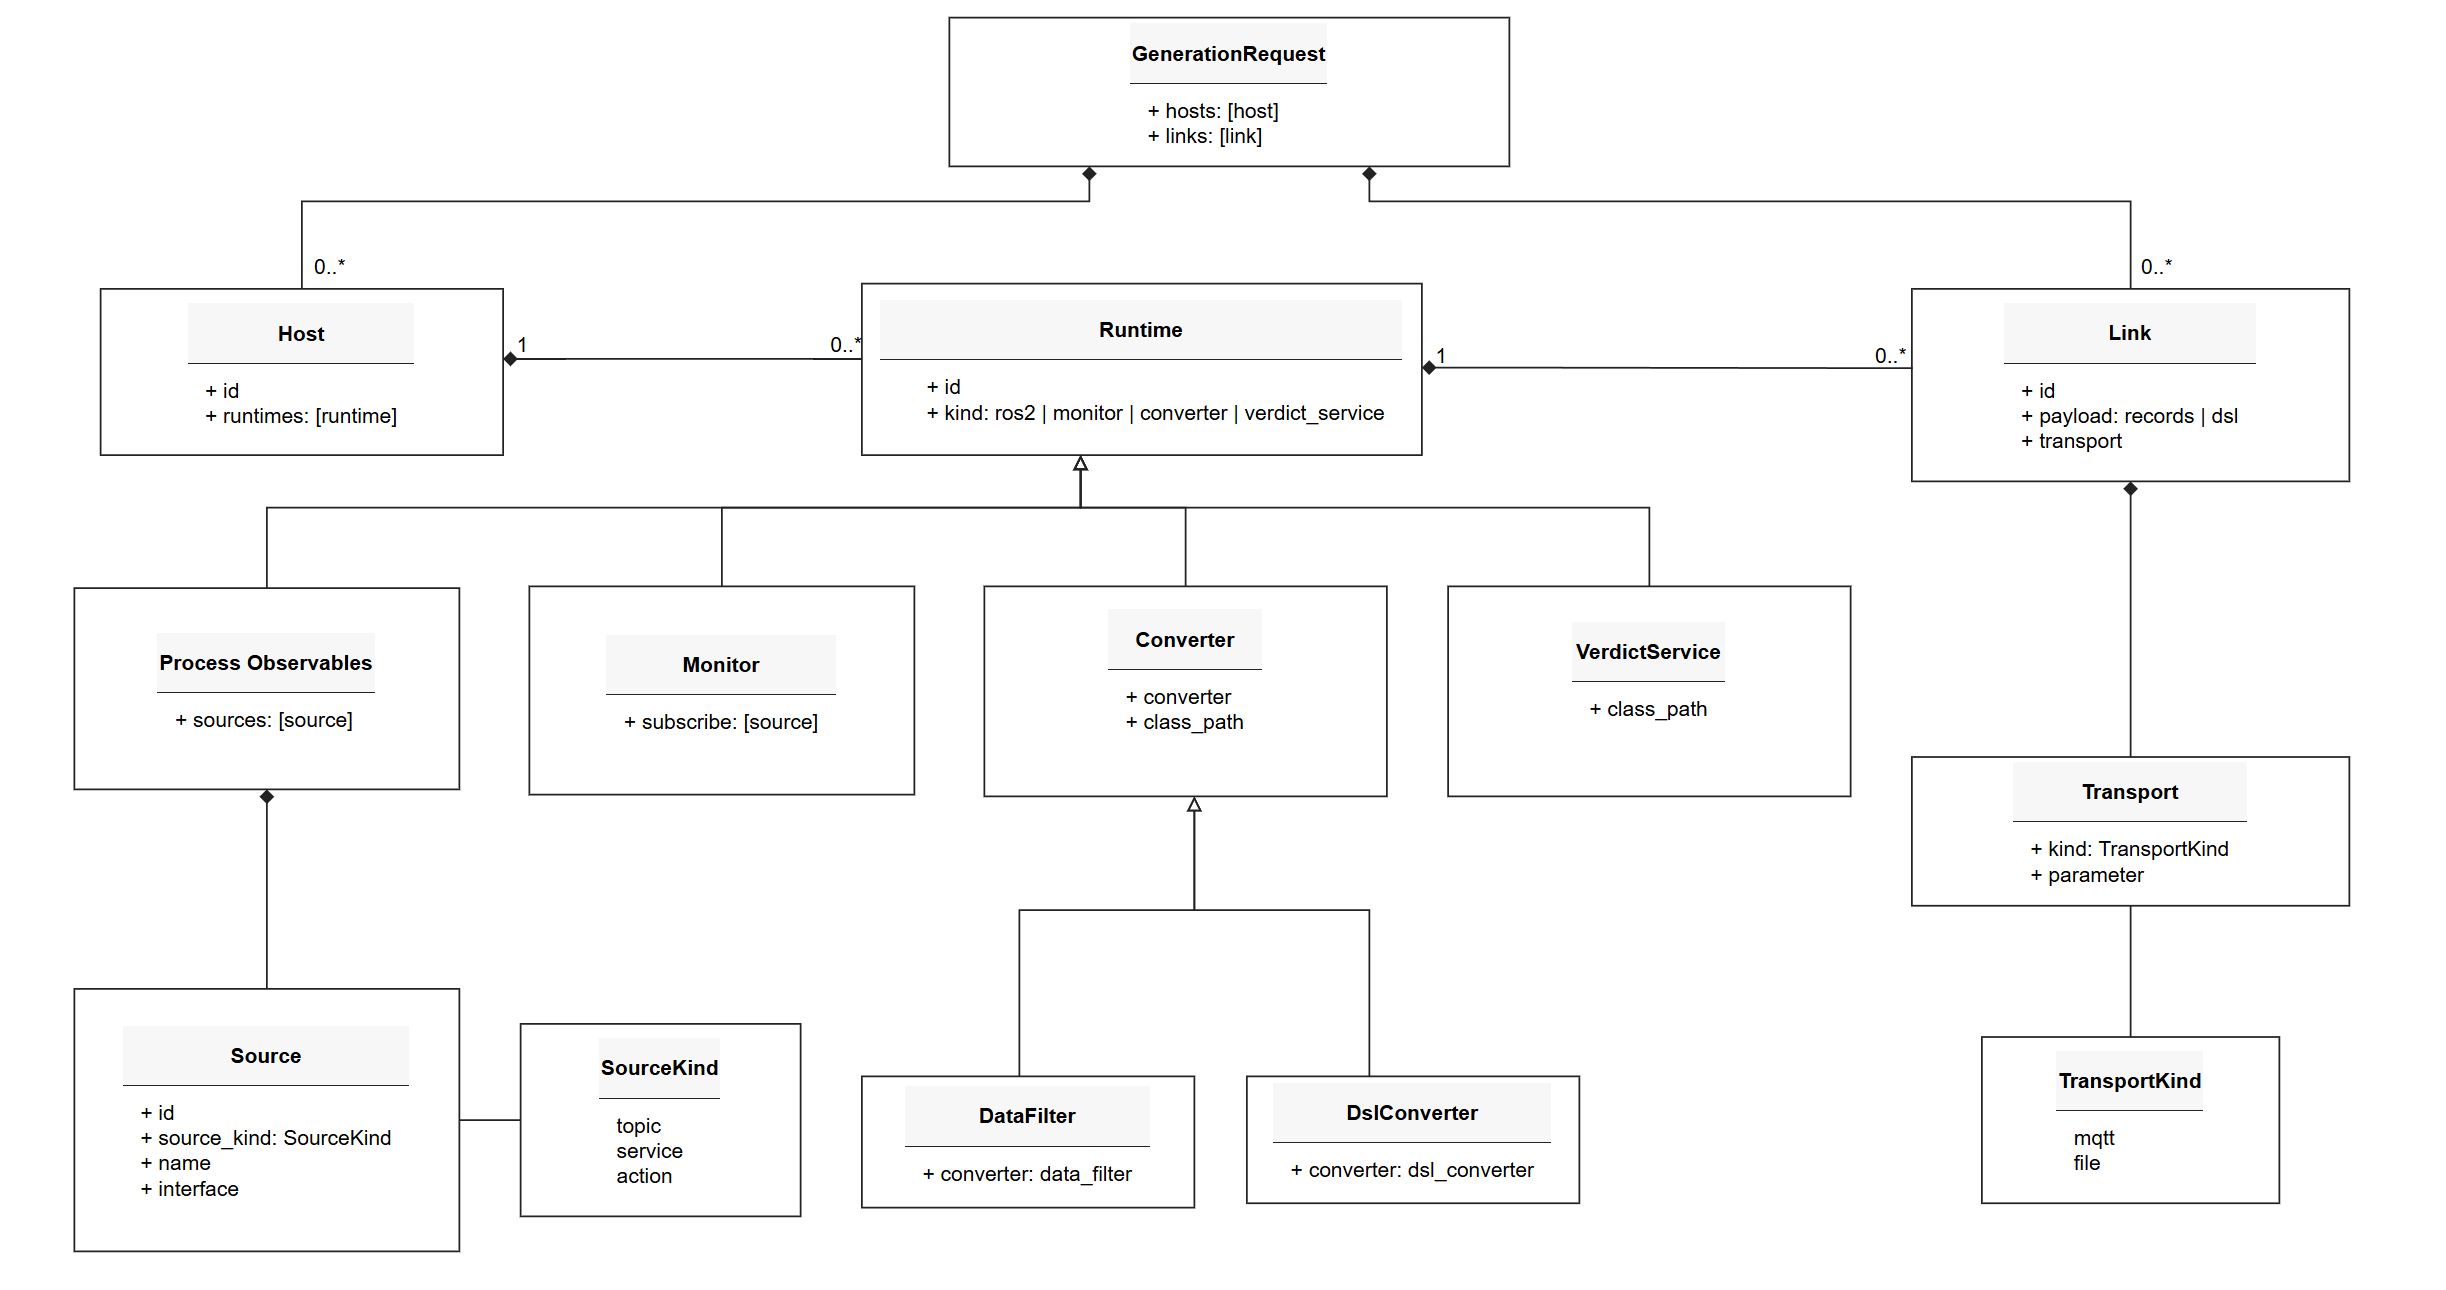
\includegraphics[width=\textwidth]{diagrams/CodeGen.png}
    \caption{Data model used by the configuration generator. A generation
    request contains hosts and links. Hosts contain runtimes, process
    observables declare monitorable sources, and links define the transport
    used between runtimes.}
    \label{fig:config-generation-model}
\end{figure}

The following example places a monitor next to the robot and the checking
chain on a separate verifier host:

\begin{small}
\begin{verbatim}
{"hosts": [
   {"id": "robot", "runtimes": [
      {"id": "app", "kind": "ros2", "sources": [
         {"id": "odom", "source_kind": "topic", "name": "/odom",
          "interface": "nav_msgs/msg/Odometry"}]},
      {"id": "mon", "kind": "monitor", "subscribe": ["odom"]}]},
   {"id": "verifier", "runtimes": [
      {"id": "conv", "kind": "converter",
       "class_path": "custom.rule_based:RuleBasedConverter",
       "input_from": ["odom"], "output_to": "speed", ...},
      {"id": "check", "kind": "verdict_service",
       "class_path": "custom.threshold:ThresholdVerdict",
       "input_from": ["speed"], ...}]}],
 "links": [
   {"from_host": "robot", "to_host": "verifier",
    "from_runtime": "mon", "to_runtime": "conv",
    "payload": "records",
    "transport": {"kind": "mqtt", "broker": "192.168.1.10"}}]}
\end{verbatim}
\end{small}

Algorithm~\ref{alg:config-generation} shows the projection used by the
generator. The algorithm first builds an index of sources, runtimes, host
placement, and cross-host links. It then emits at most one YAML file per host:
a monitor configuration for a host with a monitor runtime, or a runner
configuration for a host that only runs checking components.

\begin{algorithm}[htbp]
\caption{Project a deployment request into runtime YAML files}
\label{alg:config-generation}
\begin{algorithmic}[1]
\Require deployment request $J$
\Ensure generated configurations $F$
\State $F \gets \emptyset$
\State $I \gets \Call{BuildIndex}{J.\text{hosts}, J.\text{links}}$
\ForAll{host $H$ in $J.\text{hosts}$}
  \State $K \gets$ the set of runtime kinds on $H$
  \If{\texttt{monitor} is in $K$}
    \State $Y \gets \Call{NewMonitorConfig}{H}$
    \ForAll{monitor runtime $M$ on $H$}
      \State $E \gets \Call{RecordExporters}{M,I}$
      \ForAll{source id $s$ in $M.\text{subscribe}$}
        \State add $\Call{SourceEntry}{I.\text{sources}[s],E}$ to $Y$
      \EndFor
    \EndFor
    \State $G \gets \Call{NewGraphSection}{H,I}$
    \ForAll{converter runtime $C$ on $H$}
      \State reject unsupported cross-host record inputs to $C$
      \State $\Call{AddConverter}{G,C}$
    \EndFor
    \ForAll{verdict-service runtime $V$ on $H$}
      \State reject unsupported cross-host DSL inputs to $V$
      \State $\Call{AddVerdict}{G,V}$
    \EndFor
    \State $\Call{ApplyGraph}{G,Y}$
    \State $F[H.\text{id}] \gets Y$
  \ElsIf{$K$ contains \texttt{converter} or \texttt{verdict\_service}}
    \State $Y \gets \Call{NewRunnerConfig}{H}$
    \State $G \gets \Call{NewGraphSection}{H,I}$
    \ForAll{converter runtime $C$ on $H$}
      \State add incoming cross-host record inputs for $C$
      \State $\Call{AddConverter}{G,C}$
    \EndFor
    \ForAll{verdict-service runtime $V$ on $H$}
      \State add incoming cross-host DSL inputs for $V$
      \State $\Call{AddVerdict}{G,V}$
    \EndFor
    \State $\Call{ApplyGraph}{G,Y}$
    \State $F[H.\text{id}] \gets Y$
  \EndIf
\EndFor
\State \Return $F$
\end{algorithmic}
\end{algorithm}

The generator projects this description onto one YAML file per host. A host
with a monitor runtime receives a monitor-process configuration. A host with
only converters or verdict services receives a runner configuration. The
generator produces files only for hosts that run monitoring roles.

Runtimes on the same host are wired in-process by matching their declared
record identifiers. Cross-host communication requires an explicit link. The
writer and reader of a link derive their transport namespace from the same
link identity, so they use matching MQTT topics or shared file paths. Unsupported
placements are rejected during generation. The runner runtime handles all
cross-host record inputs.

For repeatable deployment, the repository also provides a container image
based on a ROS~2 base image. The image packages the monitor, the custom
components, and their dependencies. A Docker Compose service runs the monitor
on the host network so that DDS discovery can reach the robot nodes.
